
\chapter{Introduction}
\label{ch:intro}
%% -----------------------------------------------------------------------------
%% -----------------------------------------------------------------------------
\section{Motivations}
Statistical data mining techniques, such as artificial neural networks (ANN), serve to address limitations of the current catalyst development and optimization approaches (e.g., careful catalyst synthesis, characterization, and reactivity studies, combined with detailed density functional calculations). Data mining techniques in conjunction with large catalytic data sets, should be able to assist in identifying meaningful materials descriptors, trends in catalytic reactivity (scaling relations) and mechanistic differences between catalysts. This document details the exploration of these ideas for the water-gas shift (WGS) reaction (i.e., \ce{CO + H2O <--> CO2 + H2}).
%% -----------------------------------------------------------------------------
%% -----------------------------------------------------------------------------
\section{Machine Learning Fundamentals}
Data mining, the process of identifying patterns in large datasets, is a subfield of computer science at the intersection of statistics and machine learning (ML). Data mining algorithms enable computers to make predictions for complex, highly dimensional problems based on previously-encountered data. This project employs the use of artificial neural networks (ANN). ANNs are similar to traditional curve-fitting tools, which define an input-output relationship. However, ANNs differ from traditional curve-fitting models in their ability to fit highly dimensional datasets, such as those encountered in the field of catalysis. 

When developing an ANN, the model must first be `trained' using a set of examples referred to as `training data'. The training algorithm optimizes the model using training data to tune the model's mathematical parameters. While ANNs are frequently considered `black boxes', they actually consist of complex, statistically optimized mathematical functions. Trained with an appropriate data set, ANNs can be used to predict an optimum solution to a mathematically described problem. 

To place this work in the larger context of ML, the ANNs discussed in this document are a form of `supervised' ML. Each example or `instance' in the training data set consists of input information (a vector) and corresponding output information. This training data is considered `labeled' because each input instance is `labeled' with a corresponding output.

Architecturally, ANNs are similar to biological neural networks, storing and transferring information with numerical values rather than electrical impulses. Similar to a biological neural network, an ANN consists of many inter-connected `neurons' or `perceptrons', such as the one in figure \ref{fig:neuron}. For `feed-forward' networks, each neuron receives input signals from the preceding layer and sends an output signal to each neuron in the following layer \cite{Jacobson_2013}. 
	\begin{figure}[ht]
	    \centering
	    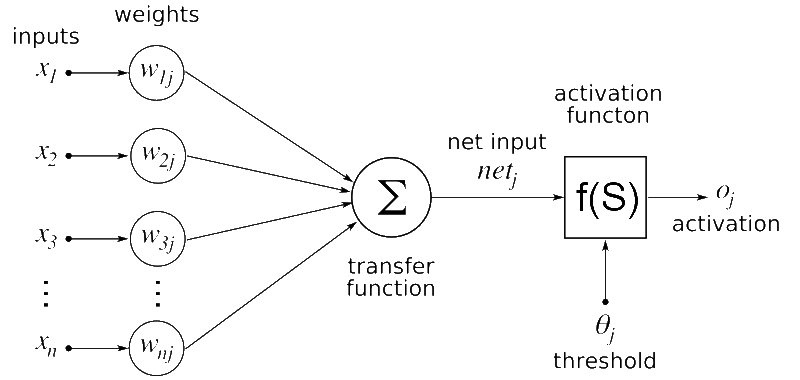
\includegraphics[width=0.6\textwidth]{Introduction/Neuron.png}
	    \caption{Example of an artificial neuron}
	    \label{fig:neuron}
	\end{figure}
Each input signal has an independent value. These input values are summed and then transformed by an `activation function' to produce a single output signal. Activation functions are typically step, linear or sigmoid functions. Mathematically, a neuron's output is determined by the activation function applied to the summation of the weighted inputs, shown in equations \ref{eq: input} and \ref{eq: output}.
	\begin{equation}
		input = w_1 x_1 + w_2 x_2 + \ldots + w_n x_n = \sum w_i x_i
		\label{eq: input} \end{equation}
	\begin{equation}
		output = f(input) = f\left( \sum w_i x_i \right)
		\label{eq: output} \end{equation}

When these neurons are linked together into a network, shown in figure \ref{fig:ANN}, the mathematical model becomes a complex function of weighted summations and activation functions. While many types of neural networks exist (i.e., deep, convolutional, relational, etc.) this report focuses on feed-forward neural networks with one or two layers of hidden neurons. Furthermore, information only travels in a forward-direction, there is no recursion or feedback within the network. The networks explored in this thesis only have a single output neuron.
	\begin{figure}[ht]
	    \centering
	    
	\begin{tikzpicture}[
			> = stealth, % arrow head style
			shorten > = 1pt, % don't touch arrow head to node
			auto,
			align=center,
			semithick, % line style
			node distance = 1mm and 2cm
		][h]

		\definecolor{awesome-grey}{RGB}{211,211,211}
		\definecolor{fantastic-grey}{RGB}{169,169,169}

		\tikzstyle{every state}=[draw = black, thick, fill = white, minimum size = 9mm]
		\tikzstyle{layer1}=[state,fill = awesome-grey]
		\tikzstyle{layer2}=[state,fill = fantastic-grey]
		\tikzstyle{invisible-border}=[state, draw = white, fill = white, minimum size = 1mm]
		\tikzstyle{inputs}=[rectangle, draw, text centered, minimum width=1.5em, minimum height=25em]%rotate around={90:(0,0)}

		% Input node is the root node positionally
		\node[inputs] (inputs) {\rotatebox{90}{Inputs}};

	% ----------------------------------------------------------------------
	% Layer 1
	% ----------------------------------------------------------------------
		% This node hides in between the Input box and layer 1 nodes for correct spacing...
		\node[invisible-border, right=0cm and 1mm of inputs] (spacing-anchor) {};

		% Nodes {x_11,x_12,x_13} are above right invisible-border
		\node[layer1, above right= of spacing-anchor] (x13) {$x_{1,3}$};
		\node[layer1, above= of x13] (x12) {$x_{1,2}$};
		\node[layer1, above= of x12, label=above:Layer 1] (x11) {$x_{1,1}$};

		% Nodes {x_14,x_15,x_16} are below invisible-border
		\node[layer1, below right= of spacing-anchor] (x14) {$x_{1,4}$};
		\node[layer1, below= of x14] (x15) {$x_{1,5}$};
		\node[layer1, below= of x15] (x16) {$x_{1,6}$};

		% Edges from input box -> {x_11,x_12,x_13,x_14,x_15,x_16}
		\path[->] (inputs) edge node {} (x11);
		\path[->] (inputs) edge node {} (x12);
		\path[->] (inputs) edge node {} (x13);
		\path[->] (inputs) edge node {} (x14);
		\path[->] (inputs) edge node {} (x15);
		\path[->] (inputs) edge node {} (x16);

	% ----------------------------------------------------------------------
	% Layer 2
	% ----------------------------------------------------------------------
		% Nodes {x_21,x_22} are above and below respectively
		\node[layer2, right= of x12, label=above:Layer 2] (x21) {$x_{2,1}$};
		\node[layer2, right= of x15] (x22) {$x_{2,2}$};

		% Edges from {x_11,x_12,x_13,x_14,x_15,x_16} -> {x_21,x_22}
		\path[->] (x11) edge node {} (x21);
		\path[->] (x11) edge node {} (x22);
		\path[->] (x12) edge node {} (x21);
		\path[->] (x12) edge node {} (x22);
		\path[->] (x13) edge node {} (x21);
		\path[->] (x13) edge node {} (x22);
		\path[->] (x14) edge node {} (x21);
		\path[->] (x14) edge node {} (x22);
		\path[->] (x15) edge node {} (x21);
		\path[->] (x15) edge node {} (x22);
		\path[->] (x16) edge node {} (x21);
		\path[->] (x16) edge node {} (x22);

	% ----------------------------------------------------------------------
	% Layer 3
	% ----------------------------------------------------------------------
		% Y and output
		\node[state, right=0cm and 7.5cm of spacing-anchor] (y) {$y$};
		\node[invisible-border, right= of y] (o) {Output};

		\path[->] (x21) edge node {} (y);
		\path[->] (x22) edge node {} (y);
		\path[->] (y) edge node {} (o);

	\end{tikzpicture}
        \caption{Simple feed-forward artificial neural network}
		\label{fig:ANN}
		\end{figure}

Consider the case with two hidden layers and a single output where the first hidden layer contains six neurons and the second layer contains two neurons, demonstrated in figure \ref{fig:ANN}.  Note that each of the neurons has the properties shown in figure \ref{fig:neuron}. To illustrate the mathematics contained in the `black box', begin by considering the output, $y$ as a function of the neurons $x_{2,1}$ and $x_{2,2}$ and their associated weights in the preceding layer, equation \ref{eq:output}. Similarly, the output from the $x_{2,1}$ and $x_{2,2}$  neurons is determined by the neurons in first hidden layer ($x_{1,1}$, $x_{1,2}$, $x_{1,3}$, $x_{1,4}$, $x_{1,5}$, $x_{1,6}$). The mathematical relationship between the first and second hidden layers is demonstrated in equations \ref{eq:x_2,1} and \ref{eq:x_2,2}. Finally, the output for each neuron in the first layer is given as a function of the network inputs ($in_1$ to $in_n$), equation \ref{eq:x_1,i}. 
		\begin{equation}
			y = f(x_{2,1}, x_{2,2}) 
			\label{eq:output}\end{equation}
		\begin{equation}
			x_{2,1} = f_{2,1}(x_{1,1}, x_{1,2}, x_{1,3}, x_{1,4}, x_{1,5}, x_{1,6}) 
			\label{eq:x_2,1}\end{equation}
		\begin{equation}
			x_{2,2} = f_{2,2}(x_{1,1}, x_{1,2}, x_{1,3}, x_{1,4}, x_{1,5}, x_{1,6})
			\label{eq:x_2,2}\end{equation}
		\begin{equation}
			x_{1,i} = f_{1,i}(in_1, in_2, \ldots, in_n)
			\label{eq:x_1,i}\end{equation}
To determine the overall function representing the ANN shown, begin by nesting the input-output functions for each layer. First, replace the $x_{2,1}$ and $x_{2,2}$ inputs in equation \ref{eq:output} with equations \ref{eq:x_2,1} and \ref{eq:x_2,2} to yield equation \ref{eq:output nested}. Then replacing the $x_{1,i}$ inputs in equation \ref{eq:output nested} with their corresponding equation \ref{eq:x_1,i} form yields the overall ANN representation in equation \ref{eq: output nested2}.
		\begin{equation}
			\begin{split}
			y = f\big[
				f_{2,1}(x_{1,1}, x_{1,2}, \ldots, x_{1,6}), \\
				f_{2,2}(x_{1,1}, x_{1,2}, \ldots, x_{1,6}) \big]
			\end{split}
			\label{eq:output nested}
			\end{equation}
		\begin{align*}
		y = f\big[
			f_{2,1} \big(
				&f_{1,1}(in_1, in_2, \ldots, in_n) \\
				&f_{1,2}(in_1, in_2, \ldots, in_n), \\
				& \ldots,\\
				&f_{1,6}(in_1, in_2, \ldots, in_n) ],\\
			f_{2,2} [
				&f_{1,1}(in_1, in_2, \ldots, in_n) \\
				&f_{1,2}(in_1, in_2, \ldots, in_n), \\
				& \ldots,\\
				&f_{1,6}(in_1, in_2, \ldots, in_n) \big)  \big] \numberthis
			\label{eq: output nested2}
			\end{align*}

In general, increasing the size of the training data set improves predictions. A common heuristic for determining the minimum size of the training data set is that there should be twice as many instances, or total data points, in the training data set as weights in the ANN \cite{Jacobson_2013}. For the most general feedforward ANN, the number of weights is determined by equation \ref{eq:num of weights}. For ANNs discussed in this work with two hidden layers and a single output, the number of weights is given by \ref{eq:specific num of weights}.
	\begin{equation}
		weights = n_{inputs}*n_{Layer1} + n_{Layer1}*n_{Layer2} + \ldots + n_{LastLayer}*n_{outputs}
		\label{eq:num of weights} \end{equation}
	\begin{equation}
		weights = n_{inputs}*n_{Layer1} + n_{Layer1}*n_{Layer2} + n_{Layer2}
		\label{eq:specific num of weights} \end{equation}
%% ----------------------------------------------------------------------------
%% -----------------------------------------------------------------------------
\section{Previous Work in Machine Learning \& \\Catalysis}
ML was initially proposed in the 1950's with backpropagation methods incorporated in 1986 \cite{Turing_1950,Rumelhart_1986}. Three years later, in 1989, Shigeharu Kito \& Tadashi Hattori pioneered ML as a tool for catalyst optimization \cite{Kito_1989}. ANNs have since been explored for optimizing materials/catalyst properties and reaction conditions as well as approximating computationally intensive calculations \cite{Omata_2004,Corma_2002,Kito_2004,Ulissi_2017}. As experimental techniques, ML methods and computational power advance, new and exciting opportunities to merge these fields develop.

	% -------------------------------------
	\subsection{Experimental Catalysis}
	The earliest and most-explored application of ML in catalysis has been in using ANNs to approximate the reactivity or selectivity for differing catalyst compositions. This movement was led by Kito \& Hattori who, in 1989, proposed INCAP (INtegration of Catalyst Activity Patterns), a system they claimed was capable of predicting the reaction mechanism, important catalytic functions, plausible side reactions, unfavorable products resulting from said side reactions and proposing catalyst candidates \cite{Kito_1989}. Kito \& Hattori continued publishing on ML in catalysis through 2006 \cite{Kito_2006}. Using ANNs they developed models to predict the acid strength of mixed oxides, predict the product selectivity for the oxidative dehydrogenation of methane, predict the catalyst deactivation in methanol conversion, and identify factors controlling catalytic activity \cite{Kito_1991,Kito_1994,Kito_2004,Kito_2006}. 

	Kohji Omata \& Muneyoshi Yamada also made significant contributions to the intersection of catalysis and ML. Together they published a series of papers exploring Radial Basis Function Networks (RBFN), which are similar to ANNs, for catalyst optimization. These networks optimized Co loading and preparation \cite{Omata_2006_1}, promoter optimization for oxidation of \ce{CO} and dry reforming of methane \cite{Omata_2009,Omata_2007,Omata_2010}. They also developed RBFNs for optimizing the preparation and composition of a Cu-Zn-Al-Sc-B-Zr catalyst for methanol synthesis, ternary-oxide Cu catalysts for steam reforming of methanol and promoters for \ce{Ni}/activated carbon catalysts for carbonylation of methanol \cite{Omata_2004,Omata_2004_2,Omata_2008}. Finally, Omata \& Yamada used RBFNs to optimize a Cu-Zn catalyst for dimethyl ether synthesis and a ZSM-5 catalyst for dimethyl ether to olefin conversion \cite{Omata_2006_2,Omata_2009_2}. For each application, their training data was largely generated `in house' using high throughput techniques. As attributes, Omata \& Yamada repeatedly chose to use chemical properties (molecular weight, boiling point, etc). However, he did not perform any analysis or optimization on the attributes chosen. 

	Finally, Avelino Corma has published on several diverse catalytic applications for ANNs and proposed a Design of Experiments framework. Corma began using ANNs to predict catalyst activity and selectivity for oxidative dehydrogenation of ethane \cite{Corma_2002}. The developed ANN used molar catalyst composition to predict reactant conversion, product yield and overall selectivity. More recently, Corma  et al. used ANNs with high throughput experimental techniques to optimize a \ce{Ti} catalyst for olefin epoxidation \cite{Corma_2005}. Additionally, they looked at ANNs and decision trees to successfully predict material properties (e.g., stability) based on composition for the high temperature synthesis of zeolites \cite{Corma_2006}. Finally, Corma et al. describe a `soft-computing framework' which combines a genetic algorithm, an ANN and high-throughput experimentation to rapidly optimize a catalyst within the defined domain \cite{Corma_2008}. Additionally, Corma has demonstrated the use of ANNs to optimize not only catalyst composition, but also reaction conditions and scale-up approaches, focusing on n-paraffin isomerization \cite{Corma_2003_1,Corma_2003_2}. 

	\subsection{Scaling Relations}

	In catalysis, scaling relations have been successfully used to drive development of novel catalytic materials and predict catalytic activity \cite{Greeley_2016}. Defining a scaling relation as any relationship in which a change to one variable causes a predictable and defined change in another variable and revisiting equations \ref{eq: output} through \ref{eq: output nested2}, it is clear that ANNs can be framed as a sophisticated scaling relationship tool. While each neuron alone performs a predictable transformation on its inputs, the network as a whole also fits within the definition of a scaling relationship. 

	Currently, scaling relations for heterogeneous catalysis relate elementary step activation energies to adsorption energies and thus reactivity of key intermediates \cite{Gani_2017}. However, it is well understood that catalysts cannot demonstrate activities above the peak of the volcano plot while obeying scaling relations \cite{Andersen_2017}. Therefore, identifying materials which break scaling relations may have important implications for future catalyst development. 
	
	% -------------------------------------
	\subsection{Explored in this Work}
	This work expands on the foundational work presented by increasing the catalyst domain space, incorporating diverse training data, optimizing attribute selection and incorporating DFT-derived descriptors. The laborious effort of Odabasi, Gunay and Yildrim resulted in a database of 4,360 data points for the water-gas shift (WGS) reaction derived from publications spanning 10 years (2002 to 2012) \cite{Odabasi_2014}. The data used for this work follows from the database constructed and published by Odabasi, Gunay and Yildrim. 

	Unlike the previous ANN studies cited, which largely rely on high-throughput data from individual research groups, the data in this study was collected in numerous laboratories with diverse experimental equipment and procedures. While much of the cited literature considers only a narrow scope of catalysts (i.e., only varying a single parameter such as promoter or active metal), this thesis considers many different supports, active metals, promoters, synthesis techniques and reactor conditions. To my knowledge, this is the first study using ANNs to combine DFT attributes (binding energies) with chemical properties to predict the fundamentally-explained forward rate. Furthermore, this works begins discussion on applying ML to derive scaling relations and evaluate meaningful catalyst attributes.  

